%%%%%%%%%%%%%%%%%%%%%%%%%%%%%%%%%%%%%%%%%%%%%%%%%%%%%%%%%%%%%%%%%%%%%%
%% Validation section -- standalone working document (one page)
%% Paper: Mapping the land-use footprint of Brazilian soy embodied in
%%        international consumption -- a spatially explicit input-output
%%        approach
%%
%% Self-contained: no cross-references into methods_v2.tex; pointers to
%% the Methods appendices are given in plain text. Compile with:
%%   pdflatex validation && bibtex validation && pdflatex validation && pdflatex validation
%%%%%%%%%%%%%%%%%%%%%%%%%%%%%%%%%%%%%%%%%%%%%%%%%%%%%%%%%%%%%%%%%%%%%%

\documentclass[pdflatex,sn-nature]{sn-jnl}% Nature Portfolio reference style

\usepackage{graphicx}%
\usepackage{amsmath,amssymb,amsfonts}%
\usepackage{xcolor}%
\usepackage{textcomp}%
\usepackage{manyfoot}%
\usepackage{booktabs}%
\usepackage{geometry}%
\geometry{textheight=240mm}%
\usepackage{float}%
\raggedbottom

\begin{document}

\title[Validation]{Validation (working document)}

\author*[1]{\fnm{Liza} \sur{Buriak}}\email{TODO@wu.ac.at}

\affil*[1]{\orgdiv{Institute for Ecological Economics},
\orgname{Vienna University of Economics and Business (WU)},
\orgaddress{\city{Vienna}, \country{Austria}}}

\abstract{Standalone draft of the Validation section. The text is
self-contained; appendix pointers refer to the Methods working document
(methods\_v2).}

\maketitle

%%%%%%%%%%%%%%%%%%%%%%%%%%%%%%%%%%%%%%%%%%%%%%%%%%%%%%%%%%%%%%%%%%%%%%
\section{Validation}\label{sec:validation}
%%%%%%%%%%%%%%%%%%%%%%%%%%%%%%%%%%%%%%%%%%%%%%%%%%%%%%%%%%%%%%%%%%%%%%

\subsection{Agreement with the Trase benchmark}\label{subsec:val-trase}
The reconstructed origin-to-importer flows are evaluated against the
independent Trase Brazil--soy dataset (v2.6.1), which links
municipalities of production to countries of first import using
per-shipment customs and logistics records
\cite{godar2015sei,escobar2020trase}. All three allocation variants are
compared against this benchmark on the
municipality$\times$destination flow matrix: the downscaling baseline,
the Euclidean model and the multimodal transport variant. Pooled over
all flows the three perform comparably, with mean correlations of 0.71,
0.69 and 0.69 over 2010--2022. The value added by the supply-chain
structure shows at the destination level: the mean per-destination
correlation is 0.41 for the Euclidean model and 0.42 for the multimodal
variant, against 0.28 for downscaling. Sample construction and metrics
are given in the validation appendix of the Methods document.

\subsection{Agreement grows with flow size}\label{subsec:val-volume}
Pooled over the 127{,}862 matched
municipality$\times$destination$\times$year flows, the log-flow
correlation with Trase is 0.68 and 54\% of the flows fall within a
factor of three of the benchmark value. In the upper half of the volume
distribution (flows above 1.2\,kt, which carry 98\% of the benchmark
tonnage) the within-factor-three share rises to 56\% and the median
deviation falls from a factor of 2.7 to 2.4; per destination, the mean
correlation rises from 0.29 in the lower half of import volumes to 0.53
in the upper half. The tonnage that carries the footprint is therefore
also the best-validated part of the flow distribution, and below roughly
$10^3$\,t per destination subnational modelling adds no information over
downscaling. This motivates the volume floor of the reporting rule:
model subnationally above the floor, downscale below it, and read
individual small-volume destinations with caution.

\subsection{Backend consistency over time}\label{subsec:val-backend}
Before 2010 the pipeline runs on FABIO v1.1 inputs instead of the v2
build. In the clean overlap years the two backends differ by 6--8\% in
the total footprint with cross-country correlations above 0.988, so
pre-2010 levels are reported unadjusted.

\subsection{Sensitivity to input assumptions}\label{subsec:val-inputs}
The two least constrained input assumptions are screened for their
effect on the benchmark agreement: the within-state location of
crushing (capacity is reported by state and the baseline divides it
equally among each state's plants) and the feed and livestock
parametrisation (per-system feed rates and the 2010 herd composition).
Twenty-four perturbed variants of the flow reconstruction are re-run
through the full chain up to the origin-to-importer flows for a
representative year (2019) and scored against Trase on the pooled
municipality$\times$destination correlation (Euclidean model, base
$r=0.72$). For the crush assumption, each state's fixed capacity total
is redistributed across its plant municipalities in proportion to
municipal soybean production or by ten seeded random draws over unknown
plant sizes, and the allocation weight is sharpened or flattened
(capacity raised to $\gamma\in\{0.5,2\}$). For the feed assumption, the
per-system bean and cake feed rates receive a lognormal jitter of
$\sigma=0.3$ across ten seeded draws (a uniform multiplier cancels in
the national rescale, so the jitter shifts only the relative system
mix), and the 2010-frozen municipal herd composition is replaced by
state-average shares.

The two assumptions separate cleanly (Table~\ref{tab:val-inputs},
Figure~\ref{fig:val-inputs}).
Crush location accounts for nearly all of the induced variation: the
random within-state splits span correlations of 0.67 to 0.74 (spread
0.073), the production-proportional split scores 0.69, and the
allocation-sharpness variants span 0.024. The feed variants are
immaterial: the ten feed-rate draws move the correlation by less than
0.01 and the herd-composition variant by less than 0.001. Agreement
with the benchmark is therefore limited by where processing sits within
states, not by the feed model, and even the widest perturbation leaves
the correlation within 0.05 of the reported value.

\begin{table}[htbp]
\caption{Input-assumption sensitivity of the model--Trase correlation
(pooled municipality$\times$destination flows, Euclidean model, 2019;
base $r=0.723$).}\label{tab:val-inputs}
\begin{tabular}{@{}llccc@{}}
\toprule
Assumption & Perturbation & Runs & $r$ range & Spread \\
\midrule
Crush location & random within-state splits & 11 & 0.671--0.744 & 0.073 \\
Crush location & allocation sharpness $\gamma\in\{0.5,2\}$ & 2 & 0.706--0.731 & 0.024 \\
Feed rates & per-system lognormal jitter ($\sigma=0.3$) & 10 & 0.717--0.725 & 0.007 \\
Herd composition & state-average system shares & 1 & 0.722 & $<0.001$ \\
\botrule
\end{tabular}
\end{table}

\begin{figure}[htbp]
\centering
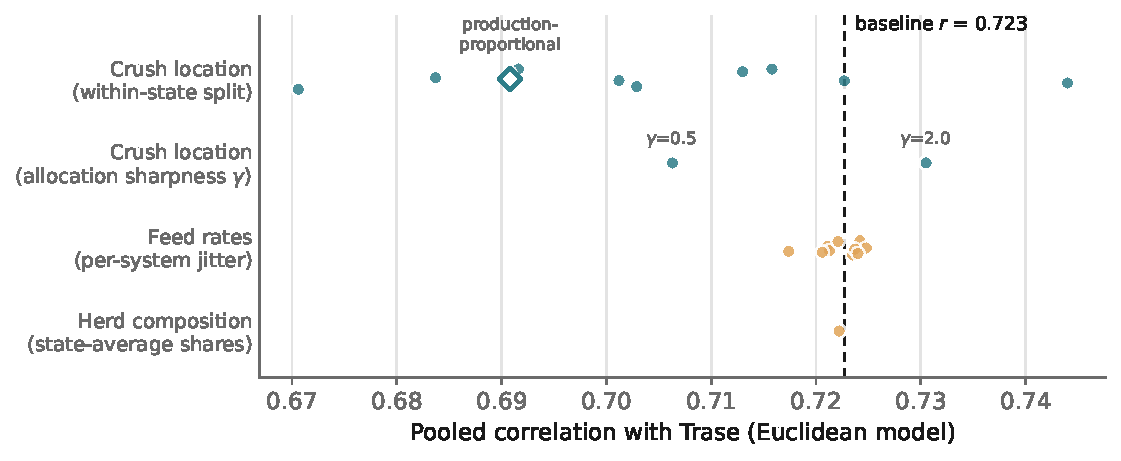
\includegraphics[width=\textwidth]{figures/fig_sens_inputs.pdf}
\caption{Input-assumption sensitivity of the model--Trase correlation.
Each dot is one perturbed re-run of the 2019 flow reconstruction, scored
against Trase on the pooled municipality$\times$destination correlation
(Euclidean model); the dashed line marks the baseline run. Crush-location
variants (teal) span the within-state capacity splits (ten seeded random
draws plus the production-proportional split, open diamond) and the
allocation-sharpness exponents $\gamma\in\{0.5,2\}$; feed variants
(orange) span ten seeded per-system feed-rate jitters and the
state-average herd composition. Vertical scatter within a row is jitter
for legibility only.}\label{fig:val-inputs}
\end{figure}

\bibliography{refs}%

\end{document}
